\chapter{Artificial Racing Agent}
\label{chapter:agent}

In this chapter we will first analyze how human racing drivers approach the task of car racing. We will then use this information to design a behavior of an autonomous agent and decompose the problem into several smaller tasks. We will discuss how we can analyze the racing track and prepare it for trajectory planning.

\section{Racing Line}
\label{sec:racing_line}

When a human driver drives on a racing circuit, his or her task is to complete several laps around the circuit in a time period as short as possible. In order to minimize the lap times, the driver trades off the total distance the car travels for the average speed at which it moves. The trajectory of the vehicle through the racing track is sometimes referred to as the racing line and it depends on the shape of the track and on the vehicle. The driver will follow different racing lines for different vehicles on the same circuit based on many their different properties such as maximum speeds, acceleration, braking power, or the grip of the tires.

For a turn with a steady curvature there is a maximum speed at which a specific car can go and stay on the track. Exceeding this speed will cause a loss of friction between the tires and the road surface and the tires will not be able to exert enough lateral force to keep the car on the curve and the car will start to travel along a curve with a greater radius than the one commanded by the driver. This situation is called understeer or oversteer, depending on whether it was the front or rear wheels which lost the friction and which wheels are powered by the engine.

\begin{figure}
	\label{fig:oversteer_understeer}
	\missingfigure{Understeer vs. oversteer}
	\caption{This figure shows the difference between oversteer and understeer.}
\end{figure}

On the other hand, for a constant vehicle speed, the vehicle can safely travel along any curve with a radius greater than the minimum safe radius. The driver will therefore try to follow curves with higher radii when going through corners but only to the point where the maximum safe speed reaches the maximum speed of the vehicle. Increasing the curvature when it is not possible to increase the speed adds to the distance the car travels but it does not increase the average speed and therefore leads to a higher lap time.

The trajectory of the vehicle as it goes through a corner can be split into several stages. First, the vehicle aligns itself to the outer edge of the track. Second, the vehicle must adjust its speed so it can safely stay on the curve. It is common to use the brakes mostly while the vehicle is moving straight to avoid locking the wheels in mid-turn. Third, the car starts turning at a turn-in point to go through the apex of the curve at the desired moment. Fourth, the vehicle goes through an apex, which is the point, where it is the closest to the inner edge of the track. Next, the vehicle starts exiting the corner and enters another part of the track.

There are two common ways of going through a corner, a classical one and one called late apex. The classical way of leaving the corner is to keep the constant curvature of the turn and to align the vehicle with the outer edge of the track. The late apex is achieved by starting to turn into the corner later and exiting the corner much closer to the inner edge of the track than the classical way. During the late apex turn, the vehicle slows down more before entering the corner and it straightens the line before hitting the apex allowing for greater exit speed. The comparison between these two lines can be seen in Figure~\ref{fig:apex}.

\begin{figure}
	\label{fig:apex}
	\missingfigure{Classical line and Late apex: https://drivingfast.net/racing-line}
	\caption{Classical line vs. Late apex}
\end{figure}

Another factor which affects the speed at which the driver can go through a corner is the shape of the track around the corner. When there is a straight stretch following the corner, the driver can maximize the speed at which the vehicle leaves the corner to increase the average speed. If there is another corner immediately after the first one, the driver must plan ahead and adjust the speed before entering the first corner to a level at which the exit speed of the first corner will be appropriate to go through the following corner.

From the description of the racing behavior of human expert drivers, it is apparent that the key components of choosing the optimal racing line are the knowledge of the behavior of the vehicle and the shape of the track. The knowledge of the track gives the driver an opportunity to plan how he or she is going to approach driving on the track. The driver can plan how to approach each individual corner and what speeds and turning radii are optimal and still safe.

\section{Artificial Agent}

\begin{defn}\label{def:rational_agent}
    A rational agent is an entity which gathers information from the environment through sensors and changes the state of the environment in order to maximize some performance measure.
\end{defn}

A racing driver can be thought of as a rational agent as defined in definition~\ref{def:rational_agent}. The driver observes the position of the vehicle on the racing track and the state of the vehicle as it moves along the track. He also observes the distance to the boundaries of the track and to any obstacles which can be present on the track. The driver reacts to these perceptions by giving control inputs to the vehicle through the steering wheel, brake and accelerator pedals, and shifting into different gears. The performance measure is the lack of collisions with the boundaries of the track or any obstacles on the track and minimizing of the lap time.

An artificial racing agent would use electronic sensors such a LIDAR, wheel encoders, an \gls{IMU}, or a camera to observe the state of the environment. Based on this observation, the agent can estimate its state in the world and the state of other entities in the world, such as obstacles or opponents. Based on this information, the agent has to select a control input for the actuators of the vehicle.

The agent can use the information about its initial state and calculate a time-optimal racing line from this initial state through the whole circuit up to the finish line using a trajectory planning algorithm. Depending on the size of the circuit, this could be a computationally expensive operation. If later on there is a need to re-plan the trajectory during the race, because the vehicle could not follow the trajectory accurately and it is necessary to come up with a contingency plan, the vehicle might have to repeat the expensive calculation. Instead, the agent can analyze the shape of the circuit and identify the corners and focus its effort only on the next two or three corners ahead of him.

\subsection{Decision Process}

An agent is sometimes described in the form of an agent function. This function takes the data from the sensors and outputs a command for the actuators. The command is then executed and it has an effect on the environment. In the next step we measure the changed state of the environment and the agent reacts to this changed state. The agent can select the next command in an order to correct the outcome of the previous command when it is different from the predicted outcome. This process is then repeated over and over in a so-called closed-feedback loop.

In order to avoid describing the logic of the racing agent in a single complicated function, we can divide the decision process of the agent into several smaller independent sub-problems: localization, track analysis and waypoint selection, trajectory planning, and trajectory following. Some of these sub-problems output information which is necessary as an input for another of these sub-problems they form nodes of a dependency graph of the decision process which is visualized in Figure~\ref{fig:racing_agent_diagram}.

There is one more reason to decompose the task into several sub-problems. The rate at which the nodes produce outputs is different and they work asynchronously. While the trajectory following node should react to any location update with an action to correct the movement of the vehicle and it should do this many times per second, the planning process of a trajectory will take some non-trivial time and so the trajectory planning node will have much lower output frequency.

\begin{figure}[]\centering
	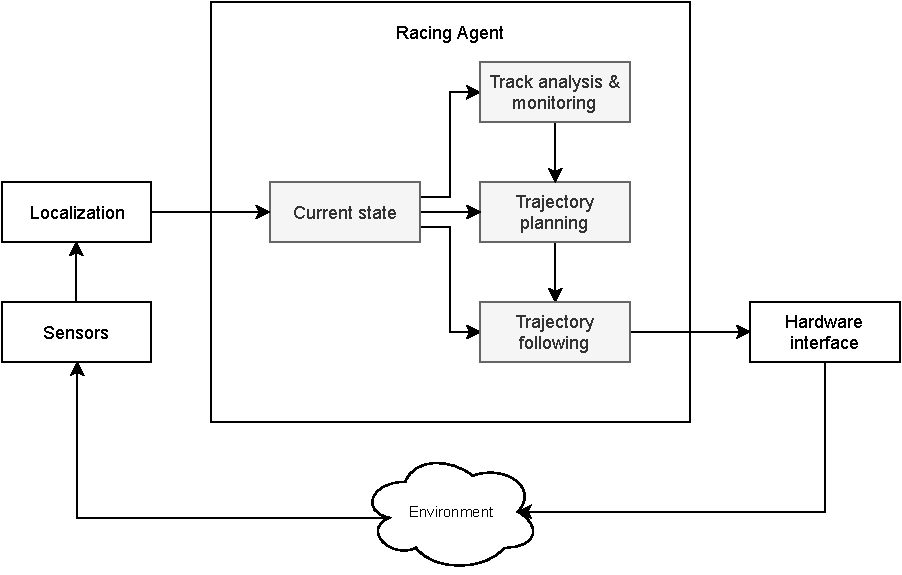
\includegraphics[width=125mm]{../img/racing_agent_diagram.pdf}
	\caption{A diagram of the decision process of the racing agent.}
	\label{fig:racing_agent_diagram}
\end{figure}

\paragraph{Current state} As the vehicle moves on the track, the agent needs to know its current state: its position on the map, orientation, and speed. A localization algorithm collects the data from different sensors and estimates the current state of the vehicle. The accuracy and the frequency of state updates depend greatly on the capabilities of the sensors and the processing power of the on-board computer. The agent takes the raw data from a localization process and produces a convenient representation of the current state for track monitoring, trajectory planning, and trajectory following.

\paragraph{Track analysis \& monitoring} Before the race begins, the agent analyses the track and finds the corners and bends on the track and marks a coordinate of a point near the apex of the corner and forms a list of waypoints along the track. During the race, the agent will keep track of which of the waypoints discovered during track analysis it drove past the last. The waypoint selection node will publish the following $n$ waypoints as the next goal for trajectory planning. The parameter $n\in\mathbb{N}$ is the lookahead of the agent. The selection of this parameter is a trade off between the quality of the trajectory and the size of the configuration space that will be search. This directly affects the update rate of the trajectory planning node.

\paragraph{Trajectory planning} The trajectory planning algorithm finds a feasible trajectory from the last state of the vehicle estimated by the localization node through the selected waypoints. The trajectory planning node will start planning a new trajectory as soon as it finishes planning the previous one. As the agent drives along the circuit and drives past a waypoint, the trajectory planning algorithm receives a new sequence of waypoints and the next trajectory it plans will account also for the next corner of the circuit within the lookahead instance. Planning can be a slow process even when we try to reduce the size of the search space as much as possible. For the practical application, the planning algorithm must update the trajectories faster than the vehicle moves through the circuit. If the agent comes to the end of an old reference trajectory and it has no update, it has to stop and wait for an update. This would obviously affect the lap time which is undesirable.

\paragraph{Trajectory following} The latest reference trajectory and the current estimate of the state of the vehicle is used to calculate the next command for the actuators of the vehicle. In the ideal case, this trajectory following node will send the commands to the hardware at the maximum possible rate which the hardware is capable of. In practice we are limited by the rate at which we receive the state estimates from the localization node. The trajectory following node is also responsible for collision avoidance either by actively guiding the vehicle around the obstacles it might hit, or by slowing down the vehicle while waiting for a new reference trajectory.

